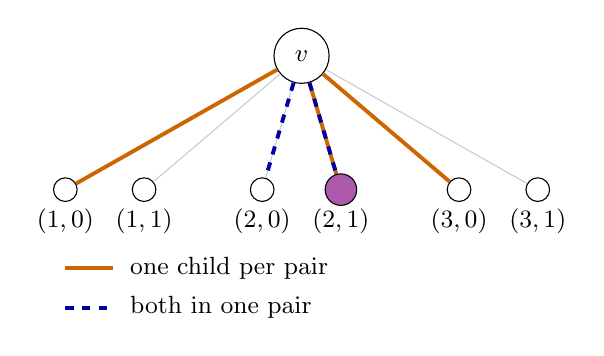
\begin{tikzpicture}[x=1cm,y=1cm,every node/.style={font=\small},
  mono/.style={draw=orange!80!black,line width=1.4pt},
  slice/.style={draw=blue!65!black,line width=1.4pt,dashed}]
\node[circle,draw,minimum size=7mm] (v) at (0,1.7) {$v$};
\foreach \x/\name/\lab in {-3/a/{(1,0)},-2/b/{(1,1)},-.5/c/{(2,0)},.5/d/{(2,1)},2/e/{(3,0)},3/f/{(3,1)}} {
 \node[circle,draw,fill=white,minimum size=3mm,inner sep=1pt] (\name) at (\x,0) {};
 \node[below] at (\x,-.12) {$\lab$};
 \draw[gray!40] (v) -- (\name);
}
\draw[mono] (v) -- (a);
\draw[mono] (v) -- (d);
\draw[mono] (v) -- (e);
\draw[slice] (v) -- (c);
\draw[slice] (v) -- (d);
\node[circle,draw,fill=violet!65,minimum size=4mm,inner sep=1pt] at (.5,0) {};
\draw[mono] (-3,-1) -- (-2.4,-1);
\node[anchor=west] at (-2.3,-1) {one child per pair};
\draw[slice] (-3,-1.5) -- (-2.4,-1.5);
\node[anchor=west] at (-2.3,-1.5) {both in one pair};
\end{tikzpicture}
